% !TEX root = main.tex
\section{Implementation of a Dataflow Library in QL for SSA-dIMP}

In this section, we describe an implementation of the algorithm schema described in the
last section.
The implementation is written in QL.
As part of the project, we implemented a library and a database scheme for SSA-dIMP.
On top of that, the dataflow algorithm is implemented.

The implementation itself is very easy, but the structure follows the
dataflow library used for Java.
It is useful, because it demonstrates how to bridge the gap between
the theoretical description of the algorithm with the soundness proof
as in \autoref{sec:df-theory} and the actual implementation of dataflow
in QL for languages like Java.
However, all the features that complicate the dataflow library for Java have been 
omitted.
The most complicated feature is that the Java dataflow library supports tracking 
flow through fields, i.e.\ if a variable that received data from a source 
is assigned to a field in an object, and a sink later reads from that field,
dataflow is detected.
Furthermore, the Java dataflow library is an interprocedural analysis.
Thus, the implementation has to be done very carefully to exhibit good
performance on large projects.

\subsection{The Database Scheme}
The database scheme is given in full in the \hyperref[lst:dbscheme]{appendix}.
The database contains a representation the abstract syntax tree (AST) of the program.
For each arithmetic expression, its unique ID, its kind
(i.e.\ integer literal, addition, multiplication, \ldots) 
and the ID of the type of the expression are saved.
Furthermore, another table contains the parent-child relation for arithmetic 
expressions - every tuple there contains the ID of an expression parent 
(either an arithmetic expression, a Boolean expression or a statement),
the ID of the child arithmetic expression and the index.
For example the addition $a_0 + a_1$ has as first child the ID of the expression 
$a_0$, and as second child the ID of the expressions $a_1$.
The order of these is an implementation detail of the database scheme in combination
with the extractor (that writes the database) and the standard library 
(that is built on top of the database scheme).

A similar database layout is employed for statements and Boolean expressions.
Expressions like literals have another relation that tracks the actual value of the
literal, variable reads have a relation that tracks the variable that is read,
variable assignments have a relation that tracks the variable that is assigned to, etc.

The database scheme is quite close how a compiler would model an AST for SSA-dIMP.
It is certainly inspired by the QL database scheme for Java.
There is one crucial difference though - in SSA-dIMP the AST is already in SSA form,
and we assume that sets $\Gamma, \Delta$ exist to prove that.
Programs in Java are not in SSA form.
Thus, as part of the QL library for Java, there exists an SSA construction algorithm
that synthesizes an SSA form.
As this is computed on the fly, it is not represented in the database scheme.

Essentially, this makes the implementation of the library for SSA-dIMP easier,
as we dont have to deal with the SSA construction.
Constructing the SSA form of a program is a well-researched problem in compiler
construction, so we feel confident that assuming the existence of an SSA form 
of the program does not lower the value of this project.

\subsection{The Standard Library}
The standard library for SSA-dIMP is implemented in the file \hyperref[lst:library]{library.qll}.

The standard library offers an object-oriented interface on top of the relational
database scheme.
Again, this interface is inspired by the corresponding library for Java.

The library offers interfaces for arithmetic expressions, and each kind of expression
has a sub-class available in the standard library.
As the QL language requires toString predicates on all classes,
the standard library also provides pretty-printing for the entire AST.

Furthermore, for example the class representing a Variable offers access to the
reads of that variable (phi nodes and variable access expressions), as well
as access to the statements that assign to this variable.
Also, the parent-child relation is exposed, and used to implement named helper predicates.
For example, for an if statement, the child branches are exposed as \texttt{getThenBranch()}
and \texttt{getElseBranch()}.
This hides the implementation detail that the then branch is the first child of the
if statement, and the else branch the second.

\subsection{The Dataflow Algorithm}
As the algorithm in \autoref{sec:df-theory} computes a type for all expressions and statements in the program,
it implicitly runs on the AST.
However, typing the whole program, while nice from the theoretical perspective, is 
inefficient if we want to only detect the possibility of dataflow.

The algorithm in practice as given in \hyperref[lst:dataflow]{dataflow.qll} runs on a subset of the AST.
Furthermore, it uses a graph structure we call the \emph{dataflow graph} to keep
track of which expressions and statements potentially get data from a source.
The nodes of that graph are made up by all expressions of kind variable access and source,
statements and phi nodes of the program.
We can restrict the node set to these expression kinds, as all other expression kinds
are always tagged with $\lclean$, and thus never take part in a dataflow computation.
The node set contains  exactly the relevant elements of the AST that are involved in determining
if a program has dataflow or not.

We can understand the typing problem as a graph problem, as
dataflow always includes two (different) steps - there has to be a source at which 
the tracked value is introduced, and there has to be a sink which reads the tracked value.
Without either, the program is safe.

We define the \texttt{flowStep} relation on the node set.
It contains the tuple $(\textit{node1}, \textit{node2})$ if \textit{node2} is using
data from the node \textit{node1}.
It can be understod as the edge set of the dataflow graph and implements the
essence of the typing rules.
A big difference to the typing rules is that we do not distinguish between $\ltracked$ and $\lunknown$.
We only have one kind of edge that indicates that data potentially flows 
from one node to another.
This means that if an expression node has type $\ltracked$ or $\lunknown$,
all downstream expression nodes on a path from the first expression node 
have type either $\ltracked$ or $\lunknown$.
Thus, the edges of the dataflow graph indicate along which paths dataflow tracking propagates
throughout the program.
We combine this propagation information with the location of the sinks and sources 
to detect potential dataflow.

By looking at the typing rule for statements, we see that only assign and sink statements
use the tracking marker assigned to the arithmetic expression used in that statement.
Thus, there is an edge from the right-hand side of an assignment (the expression) 
to the node for the assign statement, as well as from the operand from the sink 
to the node for the sink statement.

The other cases in \texttt{flowStep} take care of tracking variables.
By looking at the typing rule for expression, we see that only expressions that possibly 
result in a non-clean marker are source expressions and variable reads.
Sources are ignored in \texttt{flowStep}, because we do not care
if something flows to a source, as the result will always have a tracked marker anyways.
Thus, sources are not handled in \texttt{flowStep} at all, and only considered later.

The tracked marker for variable reads is fully determined by the type context,
which we do not explicitly compute.
In the implicit formulation, a variable access gets the tracking marker of its definition,
which is, because the program is in SSA form, unique.
If the variable definition is an assign statement, this follows immediately from the
\textsc{DF-Assign} rule - the variable is tagged with the marker of the expression.
Thus, we have an edge from the expression node to that of the 
If the variable is defined in a $\varphi$-node, we have compute the least upper bound of 
both variables that make up the $\varphi$-node.
This is implicit in the algorithm, as the $\varphi$-node will have an incoming edge if 
at least one of the variables is marked with $\ltracked$ or $\lunknown$.
However, in both cases, we have flow from a variable definition (either an assign
statement or a $\varphi$-node) to a variable read (either a VarAccess expression, 
or another $\varphi$-node).

As last step, the predicate \texttt{reaches}
computes the transitive closure of \texttt{flowStep}, beginning with all nodes
that are source expressions.
Thus, as sources are always marked with $\ltracked$ and paths in the dataflow
graph indicate that the tracked status propagate along these paths, any path 
from a source to a sink indicates the presence of (possible) dataflow.
Or, in terms of the soundness guarantee, the absence of any of these paths 
implies that the program does not contain dataflow.

\subsubsection*{On the Relation of the Algorithm to the DF Typing Rules}
As explained above, this algorithm runs already on SSA-dIMP, not dIMP.
Thus, we assume that the SSA construction already took place.
As explained in TODO, any dIMP program can be transformed into an equivalent
SSA-dIMP program.
This transformation also (implicitly) takes care of the concrete semantics of e.g.\ 
while and if statements - the dataflow algorithm only expects correctly placed $\varphi$-nodes,
and does not depend on the semantics of the individual statements.

If, for example, a repeat-until loop construct would be added to the language,
SSA-dIMP could be easily extended with that loop construct by adding a new statement 
kind to the database and implementing the library.
However, the dataflow algorithm itself would work without any changes, assuming that
the $\varphi$-node placement is correct.
This is very different from the algorithm schema above, that depends intimately on the 
typing schema, and this might be puzzling at first.
This apparent contradiction can be resolved by seeing that the DF typing 
rules serve two purposes - first, they are a refinement of the SSA typing rules,
and second, they describe an approximation on where dataflow occurs.

As the dataflow algorithm as presented here assumes that the program is already in 
SSA form, it can do substantially less than what is described in the DF rules.
In particular, it only has to worry about the introduction of flow in expressions,
and the propagation of the tracked marking to variable stores and to sinks.
Thus, it can safely skip the entire part of the rules that deal with scoping.

\subsubsection*{Example}
At last, we show the dataflow graph for the example program(\autoref{fig:ssa-dimp-example}).
Note that nodes without edges are \emph{not} included to keep the graph at a manageable size.
Node types (expression, $\varphi$ or statement) are not indicated, but are obvious from context.
Furthermore, the place of the variable accesses in the AST is only indicated when it is 
not clear from the context.

TODO add note that there is dataflow

TODO second example without flow, show how to recover "blue" typing from that

TODO modify analysis to include unknown/for sure 

TODO call SSA-dIMP structured dIMP and the other one flat/graph SSA

TODO include all dataflow node/edges

TODO strip down algorithm to not include sources
TODO ssa same name in if 
TODO source Z0

step 1 DF graph step 2 mark DF graph step 3 theorem turn marking on DF graph into safe "blue" typing

\begin{figure}[h]
    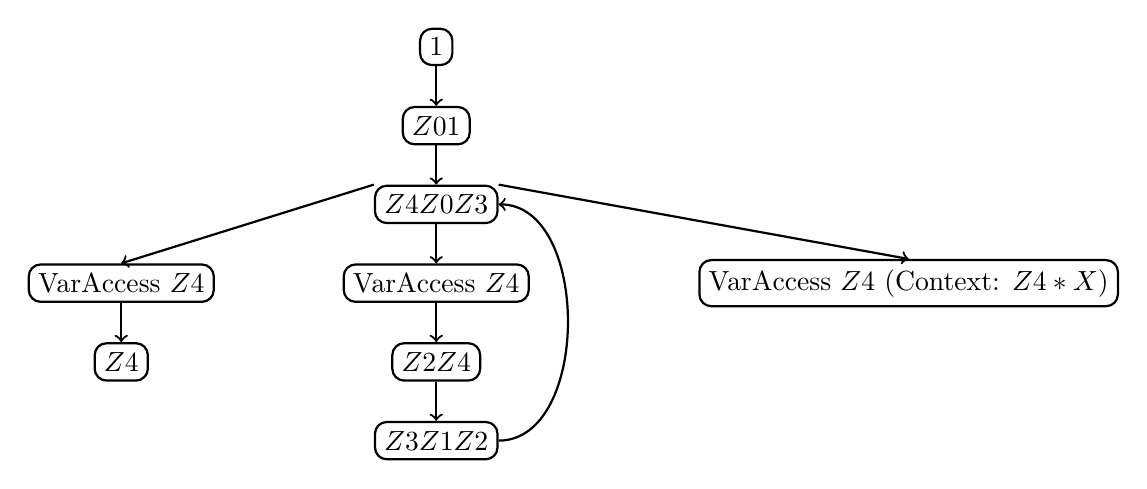
\begin{tikzpicture}[roundnode/.style={rectangle,rounded corners=1ex,draw=black!100,thick}]
        \node[roundnode] (source) at (0, 1) {$\source{1}$};
        \node[roundnode] (storez0) at (0, 0) {$\storecmd{Z0}{\source{1}}$};
        \node[roundnode] (phiz4) at (0, -1) {$\phistore{Z4}{Z0}{Z3}$};
        \node[roundnode] (mult) at (6, -2) {VarAccess $Z4$ (Context: $Z4 * X$)};
        \node[roundnode] (varaccessz4) at (0, -2) {VarAccess $Z4$};
        \node[roundnode] (storez2) at (0, -3) {$\storecmd{Z2}{Z4}$};
        \node[roundnode] (phiz3) at (0, -4) {$\phistore{Z3}{Z1}{Z2}$};
        \node[roundnode] (varaccessz42) at (-4,-2) {VarAccess $Z4$};
        \node[roundnode] (sink) at (-4,-3) {$\sink{Z4}$};
        \draw[->,thick] (source.south) -- (storez0.north);
        \draw[->,thick] (storez0.south) -- (phiz4.north);
        \draw[->,thick] (phiz4.north east) -- (mult.north);
        \draw[->,thick] (phiz4.south) -- (varaccessz4.north);
        \draw[->,thick] (varaccessz4.south) -- (storez2.north);
        \draw[->,thick] (storez2.south) -- (phiz3.north);
        \draw[->,thick] (phiz3.east) to [out=0,in=0] (phiz4.east); %.. controls(2,-2) ..
        \draw[->,thick] (phiz4.north west) -- (varaccessz42.north);
        \draw[->,thick] (varaccessz42.south) -- (sink.north);
    \end{tikzpicture}
    
    \caption{The dataflow graph for the example program}
\end{figure}


\subsection{The Query}
The query actually implementing the user-facing analysis is given in \hyperref[lst:query]{query.ql}.
It is very simple, it outputs a list of pairs of sources and sinks if the
sink is reachable from the source.
If the list is empty, the program is safe and it is guaranteed by~\autoref{thm:soundness-df}
that the program has no dataflow.
If the list is not empty, no assertion about the program correctness can be given.
